\documentclass[conference]{IEEEtran}
\IEEEoverridecommandlockouts

\usepackage[utf8]{inputenc}
\usepackage[T1]{fontenc}
\usepackage[brazil]{babel}
\usepackage{cite}
\usepackage{amsmath,amssymb,amsfonts}
\usepackage{graphicx}
\usepackage{textcomp}
\usepackage{xcolor}
\usepackage{url}
\usepackage{booktabs}
\usepackage{array}
\usepackage{listings}
\usepackage{balance}

\definecolor{codebg}{RGB}{248,248,248}
\definecolor{codekw}{RGB}{0,73,122}
\definecolor{codecm}{RGB}{82,110,72}
\definecolor{codestr}{RGB}{150,60,40}

\lstdefinestyle{homescript}{
  backgroundcolor=\color{codebg},
  basicstyle=\ttfamily\scriptsize,
  keywordstyle=\color{codekw}\bfseries,
  commentstyle=\color{codecm}\itshape,
  stringstyle=\color{codestr},
  numbers=left,
  numberstyle=\tiny\color{gray},
  numbersep=5pt,
  frame=single,
  breaklines=true,
  columns=fullflexible,
  keepspaces=true,
  showstringspaces=false,
  tabsize=2,
  morekeywords={device,sensor,pin,type,trig,echo,turn,on,off,wait,if,else,for,while,when,detected,not_detected,let,print,dispositivo,pino,tipo,gatilho,eco,ligar,desligar,esperar,se,senao,para,enquanto,quando,detectado,nao_detectado}
}

\lstdefinestyle{csmall}{
  backgroundcolor=\color{codebg},
  language=C,
  basicstyle=\ttfamily\scriptsize,
  keywordstyle=\color{codekw}\bfseries,
  commentstyle=\color{codecm}\itshape,
  numbers=left,
  numberstyle=\tiny\color{gray},
  numbersep=5pt,
  frame=single,
  breaklines=true,
  columns=fullflexible,
  keepspaces=true,
  showstringspaces=false,
  tabsize=2
}

\def\BibTeX{{\rm B\kern-.05em{\sc i\kern-.025em b}\kern-.08em
    T\kern-.1667em\lower.7ex\hbox{E}\kern-.125emX}}

\begin{document}

\title{HomeScript: uma Linguagem e um Compilador para Automação Residencial com Geração de Código C/Arduino}

\author{
\IEEEauthorblockN{Enzo Perroni\IEEEauthorrefmark{1}, João Pedro Giovanelli\IEEEauthorrefmark{2}, Arthur Schiller\IEEEauthorrefmark{3}, Arthur Camaz\IEEEauthorrefmark{4}, Maria Claudia\IEEEauthorrefmark{5}}
\IEEEauthorblockA{Curso de Ciência da Computação -- IBMEC Rio de Janeiro\\
Rio de Janeiro, Brasil\\
\IEEEauthorrefmark{1}Enzo Perroni, \IEEEauthorrefmark{2}João Pedro Giovanelli, \IEEEauthorrefmark{3}Arthur Schiller, \IEEEauthorrefmark{4}Arthur Camaz, \IEEEauthorrefmark{5}Maria Claudia}
}

\maketitle

\begin{abstract}
Este artigo apresenta o projeto HomeScript, uma linguagem de domínio específico para automação residencial e um compilador capaz de transformar arquivos \texttt{.iot} em código C/Arduino. O projeto foi desenvolvido como uma aplicação completa de conceitos de compiladores, incluindo análise léxica, análise sintática, construção de árvore sintática abstrata, verificação semântica e geração de código. Além do compilador em C, foram implementados um backend em Python com FastAPI e uma interface web em React/Vite com editor textual, visualizador de tokens, AST, código gerado e um construtor visual de automações. O objetivo é permitir que usuários descrevam comportamentos de casa inteligente com comandos simples, em inglês ou português, sem lidar diretamente com detalhes de baixo nível do Arduino.
\end{abstract}

\begin{IEEEkeywords}
compiladores, linguagem de domínio específico, automação residencial, Arduino, análise léxica, análise sintática, geração de código.
\end{IEEEkeywords}

\section{Introdução}
Automação residencial costuma exigir conhecimento de programação embarcada, elétrica básica e bibliotecas específicas de microcontroladores. Mesmo tarefas simples, como ligar uma lâmpada quando um sensor detecta movimento, normalmente envolvem escrever código C/C++ para Arduino, configurar pinos, escolher entre \texttt{digitalRead} e \texttt{analogRead}, definir \texttt{setup()} e \texttt{loop()} e tratar bibliotecas de sensores. Esse nível de detalhe cria uma barreira para usuários que entendem a regra de automação desejada, mas não dominam a implementação de baixo nível.

O projeto HomeScript foi criado para reduzir essa distância. A ideia central é oferecer uma linguagem textual simples, com extensão \texttt{.iot}, na qual o usuário declara dispositivos, sensores e regras de comportamento. O compilador então traduz essa descrição para código C/Arduino equivalente, seguindo a proposta registrada na documentação inicial do repositório~\cite{repo-readme,docs-def}. Um exemplo mínimo é apresentado na Listagem~\ref{lst:intro}.

\begin{lstlisting}[style=homescript,caption={Exemplo simples em HomeScript.},label={lst:intro}]
device luz pin 13;
sensor movimento pin 2;

when movimento == detected {
    turn luz on;
    wait 5000;
    turn luz off;
}
\end{lstlisting}

A proposta tem dois objetivos complementares. O primeiro é acadêmico: demonstrar, em um projeto funcional, as principais fases de um compilador. O segundo é de produto: criar uma interface acessível em que uma pessoa possa escrever ou montar visualmente automações e observar tokens, AST, validações e código final. A imagem de requisitos fornecida pelo professor solicita um artigo com nomes, resumo, introdução, desenvolvimento, conclusão, trabalhos futuros e referências. Este relatório segue essa estrutura usando o modelo IEEE indicado.

\section{Motivação e Pesquisa}
A motivação surgiu da observação de que regras de automação residencial possuem uma estrutura repetitiva: existem entradas, saídas, condições e ações. Em vez de exigir que cada usuário escreva manualmente código Arduino, a linguagem pode encapsular esses padrões. A pesquisa inicial considerou três pontos: sintaxe legível para leigos, correspondência direta com operações de microcontroladores e viabilidade de implementação dentro de um compilador em C.

A partir disso, a equipe definiu uma linguagem de domínio específico (DSL) com comandos próximos da linguagem natural. Declarações como \texttt{device luz pin 13;} e \texttt{sensor temperatura pin A0;} mapeiam, respectivamente, para saídas e entradas. Comandos como \texttt{turn luz on;} e \texttt{wait 1000;} mapeiam para \texttt{digitalWrite} e \texttt{delay}, que fazem parte do modelo de programação Arduino~\cite{arduino}. Estruturas \texttt{if} e \texttt{when} permitem expressar regras condicionais. Também foram adicionados sinônimos em português, como \texttt{dispositivo}, \texttt{pino}, \texttt{ligar}, \texttt{desligar}, \texttt{esperar}, \texttt{se} e \texttt{quando}, para aproximar a linguagem do público brasileiro.

A evolução do projeto foi incremental. Primeiro foram definidos tokens, regex, exemplos \texttt{.iot} e um lexer em C. Depois foram adicionados parser, AST, geração de código, análise semântica, integração com backend e uma interface web. Essa decisão reduziu risco: cada fase podia ser testada isoladamente antes de ser conectada ao pipeline completo.

\section{Visão Geral do Sistema}
A arquitetura geral do HomeScript é composta por quatro camadas: linguagem \texttt{.iot}, compilador em C, API web e frontend. A Fig.~\ref{fig:pipeline} resume o pipeline.

\begin{figure}[htbp]
\centerline{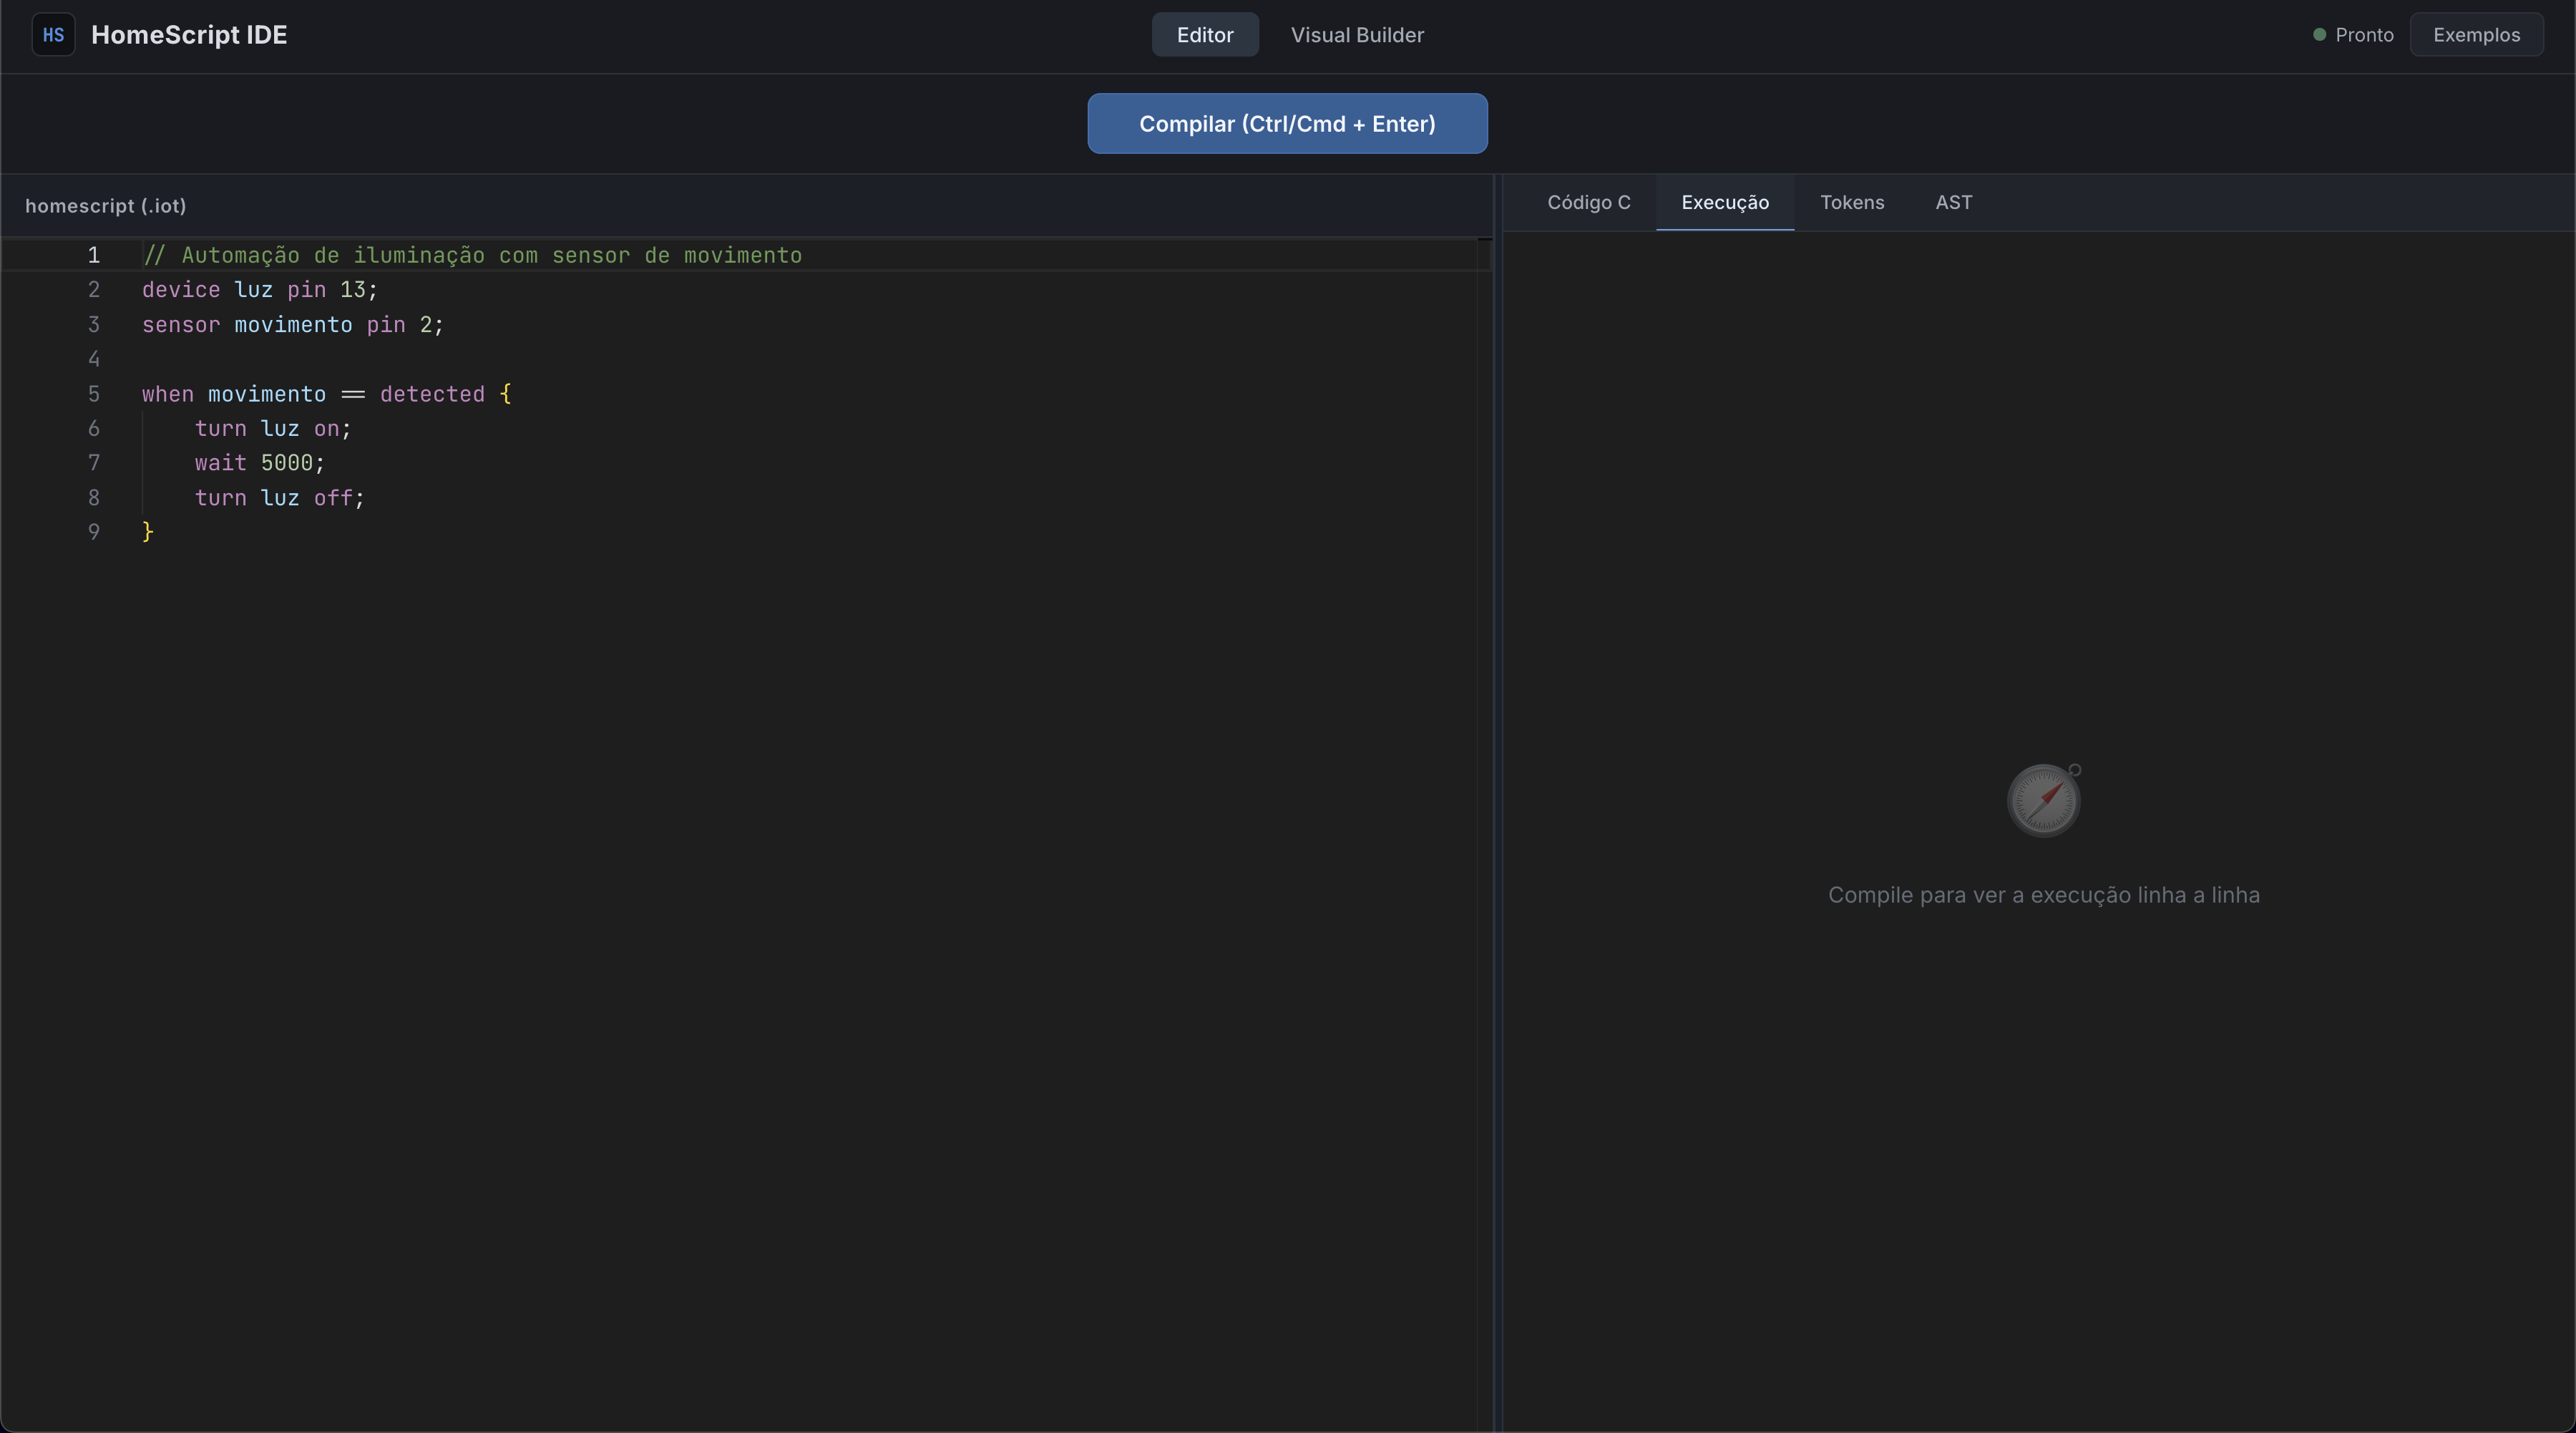
\includegraphics[width=0.95\linewidth]{../img/tela1.png}}
\caption{Tela principal da IDE HomeScript com editor, compilação e painel de resultados.}
\label{fig:pipeline}
\end{figure}

O compilador executa as fases clássicas: o lexer converte texto em tokens; o parser valida a estrutura e cria uma AST; o analisador semântico verifica nomes, tipos de entidades e uso correto de sensores; o gerador de código percorre a AST e produz C/Arduino. A API FastAPI recebe código como texto, executa o compilador em modo JSON e devolve tokens, AST, código C e erros. O frontend consome essa API e apresenta uma experiência de IDE.

\begin{table}[htbp]
\caption{Módulos principais do repositório}
\label{tab:modulos}
\centering
\begin{tabular}{p{0.25\linewidth}p{0.65\linewidth}}
\toprule
\textbf{Diretório} & \textbf{Responsabilidade} \\
\midrule
\texttt{lexer/} & Reconhecimento de tokens, posição de linha e coluna, comentários e erros léxicos. \\
\texttt{parser/} & Parser recursivo descendente, AST e impressão textual da árvore. \\
\texttt{semantic/} & Tabela de símbolos, escopos, validação de dispositivos, sensores, variáveis e pinos. \\
\texttt{codegen/} & Tradução da AST para C/Arduino, incluindo sensores genéricos, DHT11 e HC-SR04. \\
\texttt{compiler/} & CLI, opções de execução, saída normal e saída JSON. \\
\texttt{backend/} & API REST e ponte Python para executar o compilador C. \\
\texttt{frontend/} & IDE web, Monaco Editor, painéis de resultado e Visual Builder. \\
\texttt{docs/} & Especificação da linguagem, tokens, regex, storyboard e materiais de apoio. \\
\bottomrule
\end{tabular}
\end{table}

\section{Processo de Desenvolvimento}
O desenvolvimento foi dividido em etapas pequenas para que cada parte pudesse ser demonstrada separadamente. Primeiro foi criada a especificação da linguagem, com exemplos, formato de arquivo, tabela de tokens, regex e árvore hierárquica manual~\cite{docs-def,docs-tokens}. Essa etapa serviu como contrato entre o que a linguagem deveria aceitar e o que o compilador precisaria implementar.

Em seguida foi implementado o analisador léxico em C. A decisão de não usar bibliotecas externas deixou explícito o funcionamento do reconhecimento caractere a caractere. Depois disso, o parser foi adicionado para transformar a sequência de tokens em uma estrutura organizada. A AST tornou possível separar validação sintática de geração de código, evitando que o gerador dependesse diretamente de tokens soltos.

A terceira etapa foi a geração de código. Inicialmente o foco era gerar comandos Arduino simples, como \texttt{pinMode}, \texttt{digitalWrite}, \texttt{digitalRead}, \texttt{analogRead} e \texttt{delay}. Depois foram incluídos recursos mais avançados, como variáveis, expressões aritméticas, \texttt{print}, \texttt{else}, laços \texttt{for}/\texttt{while} e sensores DHT11 e HC-SR04. A quarta etapa foi a análise semântica, adicionada quando ficou claro que sintaxe correta não garantia programa correto.

Por fim, o compilador foi integrado a uma aplicação web. O backend encapsula o executável C e transforma sua saída JSON em resposta HTTP. O frontend usa React, Monaco Editor e uma tela visual para tornar o projeto demonstrável para usuários não técnicos~\cite{fastapi,react,monaco}. Essa evolução reflete a proposta dupla do projeto: ser uma entrega de compiladores e, ao mesmo tempo, parecer um produto utilizável.

\section{Definição da Linguagem HomeScript}
A HomeScript usa arquivos texto UTF-8 com extensão \texttt{.iot}. Comentários de linha começam com \texttt{//}. Comandos são encerrados por ponto e vírgula e blocos são delimitados por chaves. A estrutura típica de um programa possui declarações de dispositivos, declarações de sensores e regras.

\subsection{Declarações}
Dispositivos representam atuadores controláveis, como lâmpadas, ventiladores, sirenes ou motores. Sensores representam entradas digitais, analógicas ou componentes específicos. A sintaxe básica é:

\begin{lstlisting}[style=homescript]
device luz pin 13;
sensor movimento pin 2;
sensor luminosidade pin A0;
sensor temperatura type dht11 pin 4;
sensor distancia type hcsr04 trig 8 echo 9;
\end{lstlisting}

A versão em português aceita formas equivalentes:

\begin{lstlisting}[style=homescript]
dispositivo luz_sala pino 13;
sensor temperatura_quarto tipo dht11 pino 4;
sensor distancia_garagem tipo hcsr04 gatilho 14 eco 15;
\end{lstlisting}

\subsection{Comandos e Controle de Fluxo}
Os comandos implementados incluem ligar/desligar, espera, variáveis, atribuição, impressão serial, condicionais e laços. A linguagem suporta \texttt{if/else}, \texttt{when/else}, \texttt{while} e \texttt{for}. Em português, os equivalentes são \texttt{se/senao}, \texttt{quando/senao}, \texttt{enquanto} e \texttt{para}.

\begin{lstlisting}[style=homescript,caption={Trecho de automação residencial completa.},label={lst:complete}]
let contador_alertas = 0;

quando porta_entrada == detectado {
    contador_alertas = contador_alertas + 1;
    ligar luz_corredor;

    para i = 0; i < 3; i = i + 1 {
        ligar sirene;
        esperar 250;
        desligar sirene;
        esperar 250;
    }
} senao {
    desligar luz_corredor;
}
\end{lstlisting}

\subsection{Tokens e Expressões Regulares}
O lexer reconhece palavras reservadas, identificadores, números inteiros, pinos analógicos, operadores, delimitadores, fim de arquivo e erros. As classes foram derivadas da tabela de tokens e das expressões regulares documentadas no projeto~\cite{docs-tokens}. A Tabela~\ref{tab:tokens} resume as principais classes.

\begin{table}[htbp]
\caption{Resumo dos tokens da linguagem}
\label{tab:tokens}
\centering
\begin{tabular}{p{0.31\linewidth}p{0.27\linewidth}p{0.3\linewidth}}
\toprule
\textbf{Categoria} & \textbf{Exemplos} & \textbf{Regex ou regra} \\
\midrule
Palavras-chave & \texttt{device}, \texttt{sensor}, \texttt{when}, \texttt{if} & Verificação após identificador \\
Sinônimos PT-BR & \texttt{dispositivo}, \texttt{ligar}, \texttt{quando} & Verificação após identificador \\
Identificador & \texttt{luz}, \texttt{temp1} & \texttt{[a-zA-Z\_][a-zA-Z0-9\_]*} \\
Número & \texttt{13}, \texttt{1000} & \texttt{[0-9]+} \\
Pino analógico & \texttt{A0}, \texttt{A1} & \texttt{A[0-9]+} \\
Operadores & \texttt{==}, \texttt{!=}, \texttt{>=}, \texttt{+} & Reconhecimento com lookahead \\
Delimitadores & \texttt{\{}, \texttt{\}}, \texttt{;}, \texttt{(}, \texttt{)} & Caracteres fixos \\
\bottomrule
\end{tabular}
\end{table}

\section{Desenvolvimento do Compilador}
O compilador foi desenvolvido em C e organizado por fases. Essa separação é importante porque cada fase possui entrada e saída bem definidas, facilitando teste, manutenção e explicação pedagógica.

\subsection{Análise Léxica}
A fase léxica recebe o arquivo \texttt{.iot} e percorre caractere por caractere. O estado do lexer guarda o arquivo aberto, caractere atual, linha, coluna e indicador de fim. Antes de reconhecer cada token, a rotina pula espaços, quebras de linha e comentários de linha. Em seguida, decide qual subrotina usar: identificador/palavra-chave, número, pino analógico, operador, delimitador ou erro. O funcionamento detalhado dessa fase foi descrito no manual léxico do projeto~\cite{docs-lex}.

Um ponto relevante é o uso de lookahead na função de operadores. O caractere \texttt{=} pode representar atribuição ou compor \texttt{==}; \texttt{>} pode compor \texttt{>=}; \texttt{!} só é válido quando seguido por \texttt{=}. Essa decisão evita ambiguidade no fluxo de tokens.

\begin{lstlisting}[style=csmall,caption={Fluxo simplificado do lexer.},label={lst:lexer}]
Token lexer_proximo_token(Lexer *lexer) {
    lexer_pular_insignificantes(lexer);
    if (lexer->eof) return criar_token(TOKEN_EOF, "EOF", ...);

    char c = lexer->caractere_atual;
    if (c == 'A' && isdigit(lexer_espiar(lexer)))
        return lexer_ler_pino_analogico(lexer);
    if (isalpha(c) || c == '_')
        return lexer_ler_identificador(lexer);
    if (isdigit(c))
        return lexer_ler_numero(lexer);
    if (c == '=' || c == '!' || c == '>' || c == '<')
        return lexer_ler_operador(lexer);
    /* operadores, delimitadores e erro */
}
\end{lstlisting}

Cada token contém tipo, valor, linha e coluna. Essa informação é reaproveitada pelo parser, pela saída JSON e pelo frontend para mostrar erros localizados ao usuário.

\subsection{Análise Sintática e AST}
O parser é recursivo descendente. Ele consome tokens do lexer e cria nós da AST definidos em \texttt{parser/ast.h}. O nó raiz é \texttt{NODE\_PROGRAM}; declarações e comandos são adicionados como filhos. Condições e blocos também são nós, o que torna possível representar estruturas aninhadas.

A AST possui campos genéricos suficientes para representar nome, pino, tipo de sensor, operador, valor de comparação, estado de dispositivo, tempo de espera e expressão. Essa escolha simplifica a implementação, pois evita criar uma estrutura C diferente para cada tipo de nó, mantendo ainda a informação necessária para validação e geração de código.

\begin{lstlisting}[style=homescript,caption={Entrada usada para exemplo de AST.},label={lst:astinput}]
when movimento == detected {
    turn luz on;
}
\end{lstlisting}

A estrutura hierárquica correspondente é:

\begin{lstlisting}[basicstyle=\ttfamily\scriptsize,frame=single,breaklines=true]
Program
+-- WhenStatement
|   +-- Condition (movimento == detected)
|   +-- Block
|   |   +-- TurnCommand (dispositivo: luz, estado: ON)
\end{lstlisting}

O parser também registra erro sintático com linha, coluna, mensagem e token encontrado. Exemplos de erros tratados incluem ausência de \texttt{;}, bloco sem fechamento, comando desconhecido, \texttt{else} sem \texttt{if/when} correspondente e token inválido vindo do lexer.

\subsection{Análise Semântica}
A fase semântica foi adicionada para impedir que programas sintaticamente válidos gerem código incorreto. Ela percorre a AST, constrói uma tabela de símbolos e valida regras de consistência. Dispositivos, sensores e variáveis são registrados como símbolos. A implementação também possui controle de escopo para variáveis declaradas em blocos.

As verificações principais são: identificadores duplicados, conflito de pinos entre dispositivos e sensores, uso do mesmo pino no \texttt{trig} e \texttt{echo} do HC-SR04, acionamento de dispositivo não declarado, condição com sensor inexistente, atribuição para variável não declarada e uso de identificador desconhecido em expressão. Para o DHT11, a análise também evita comparações com \texttt{detected}, pois esse sensor deve ser usado com valores numéricos de temperatura.

Essa etapa melhora a confiabilidade da ferramenta. Sem ela, um programa como \texttt{turn bomba on;} poderia gerar \texttt{digitalWrite(bomba, HIGH);} sem que \texttt{bomba} tivesse sido declarada, causando erro posterior no compilador Arduino. Com a verificação semântica, o erro aparece diretamente na linguagem HomeScript.

\subsection{Geração de Código C/Arduino}
O gerador percorre a AST e escreve código C/Arduino em um buffer. Declarações de dispositivos viram \texttt{\#define}. Sensores genéricos viram variáveis de pino; sensores DHT11 geram objeto \texttt{DHT}; sensores HC-SR04 geram pinos \texttt{trig}/\texttt{echo} e uma função auxiliar para medir distância em centímetros.

O código gerado possui \texttt{\#include <Arduino.h>}, opcionalmente \texttt{\#include <DHT.h>}, declarações globais, \texttt{setup()} e \texttt{loop()}. Dispositivos são configurados como \texttt{OUTPUT}; sensores como \texttt{INPUT}; DHT11 chama \texttt{begin()}; HC-SR04 configura \texttt{trig} como saída e \texttt{echo} como entrada.

\begin{lstlisting}[style=csmall,caption={Exemplo de código C/Arduino gerado.},label={lst:generated}]
#include <Arduino.h>

#define luz 13
int movimento_pin = 2;

void setup() {
    pinMode(luz, OUTPUT);
    pinMode(movimento_pin, INPUT);
    Serial.begin(9600);
}

void loop() {
    if (digitalRead(movimento_pin) == HIGH) {
        digitalWrite(luz, HIGH);
        delay(5000);
        digitalWrite(luz, LOW);
    }
}
\end{lstlisting}

As condições são convertidas conforme o tipo de sensor. Para sensores digitais, \texttt{detected} vira \texttt{digitalRead(sensor\_pin) == HIGH}; \texttt{not\_detected} vira \texttt{LOW}. Para pinos analógicos, o gerador usa \texttt{analogRead}. Para DHT11, usa \texttt{readTemperature()}. Para HC-SR04, usa a função \texttt{read\_<nome>\_cm()}.

\section{Interface de Linha de Comando}
O executável principal fica em \texttt{compiler/main.c}. Ele implementa uma CLI com opções para mostrar tokens, AST, código, salvar saída em arquivo e retornar JSON. Os comandos principais são:

\begin{lstlisting}[basicstyle=\ttfamily\scriptsize,frame=single,breaklines=true]
make -C compiler
./compiler/homescript exemplos/teste.iot
./compiler/homescript exemplos/teste.iot --tokens
./compiler/homescript exemplos/teste.iot --ast
./compiler/homescript exemplos/teste.iot --code
./compiler/homescript exemplos/teste.iot --json
./compiler/homescript exemplos/teste.iot --output saida.c
\end{lstlisting}

A saída JSON foi projetada para integração com o backend. Ela inclui lista de tokens, indicador de sucesso, erro principal, lista detalhada de erros, AST serializada e código C. Essa decisão evita que a API precise interpretar saída textual formatada para humanos.

\section{Backend e Integração}
O backend foi implementado em Python com FastAPI. O arquivo \texttt{backend/app.py} define os endpoints \texttt{/compile}, \texttt{/tokens}, \texttt{/health} e \texttt{/exemplos}. O endpoint principal recebe um objeto JSON com o campo \texttt{codigo}, valida se não está vazio e chama a função \texttt{compilar}.

A ponte com o compilador está em \texttt{backend/compiler\_bridge.py}. Ela cria um arquivo temporário \texttt{.iot}, executa o binário \texttt{homescript} com a flag \texttt{--json}, captura \texttt{stdout}, interpreta o JSON e remove o temporário ao final. Também trata timeout, binário não encontrado e erro de parse JSON.

Essa separação é importante: o compilador continua sendo uma ferramenta independente de linha de comando, enquanto a API apenas o encapsula para uso web. Com isso, é possível testar o compilador diretamente ou pela interface, sem duplicar a lógica de compilação em Python.

\section{Frontend e Experiência do Usuário}
O frontend foi implementado com React, Vite e Monaco Editor, seguindo o storyboard documentado para a aplicação~\cite{docs-front}. A tela principal funciona como uma IDE: o usuário escreve código HomeScript, escolhe exemplos, compila com botão ou atalho, e visualiza código C, tokens, AST e execução passo a passo. A Fig.~\ref{fig:visual} mostra a segunda tela, o construtor visual.

\begin{figure}[htbp]
\centerline{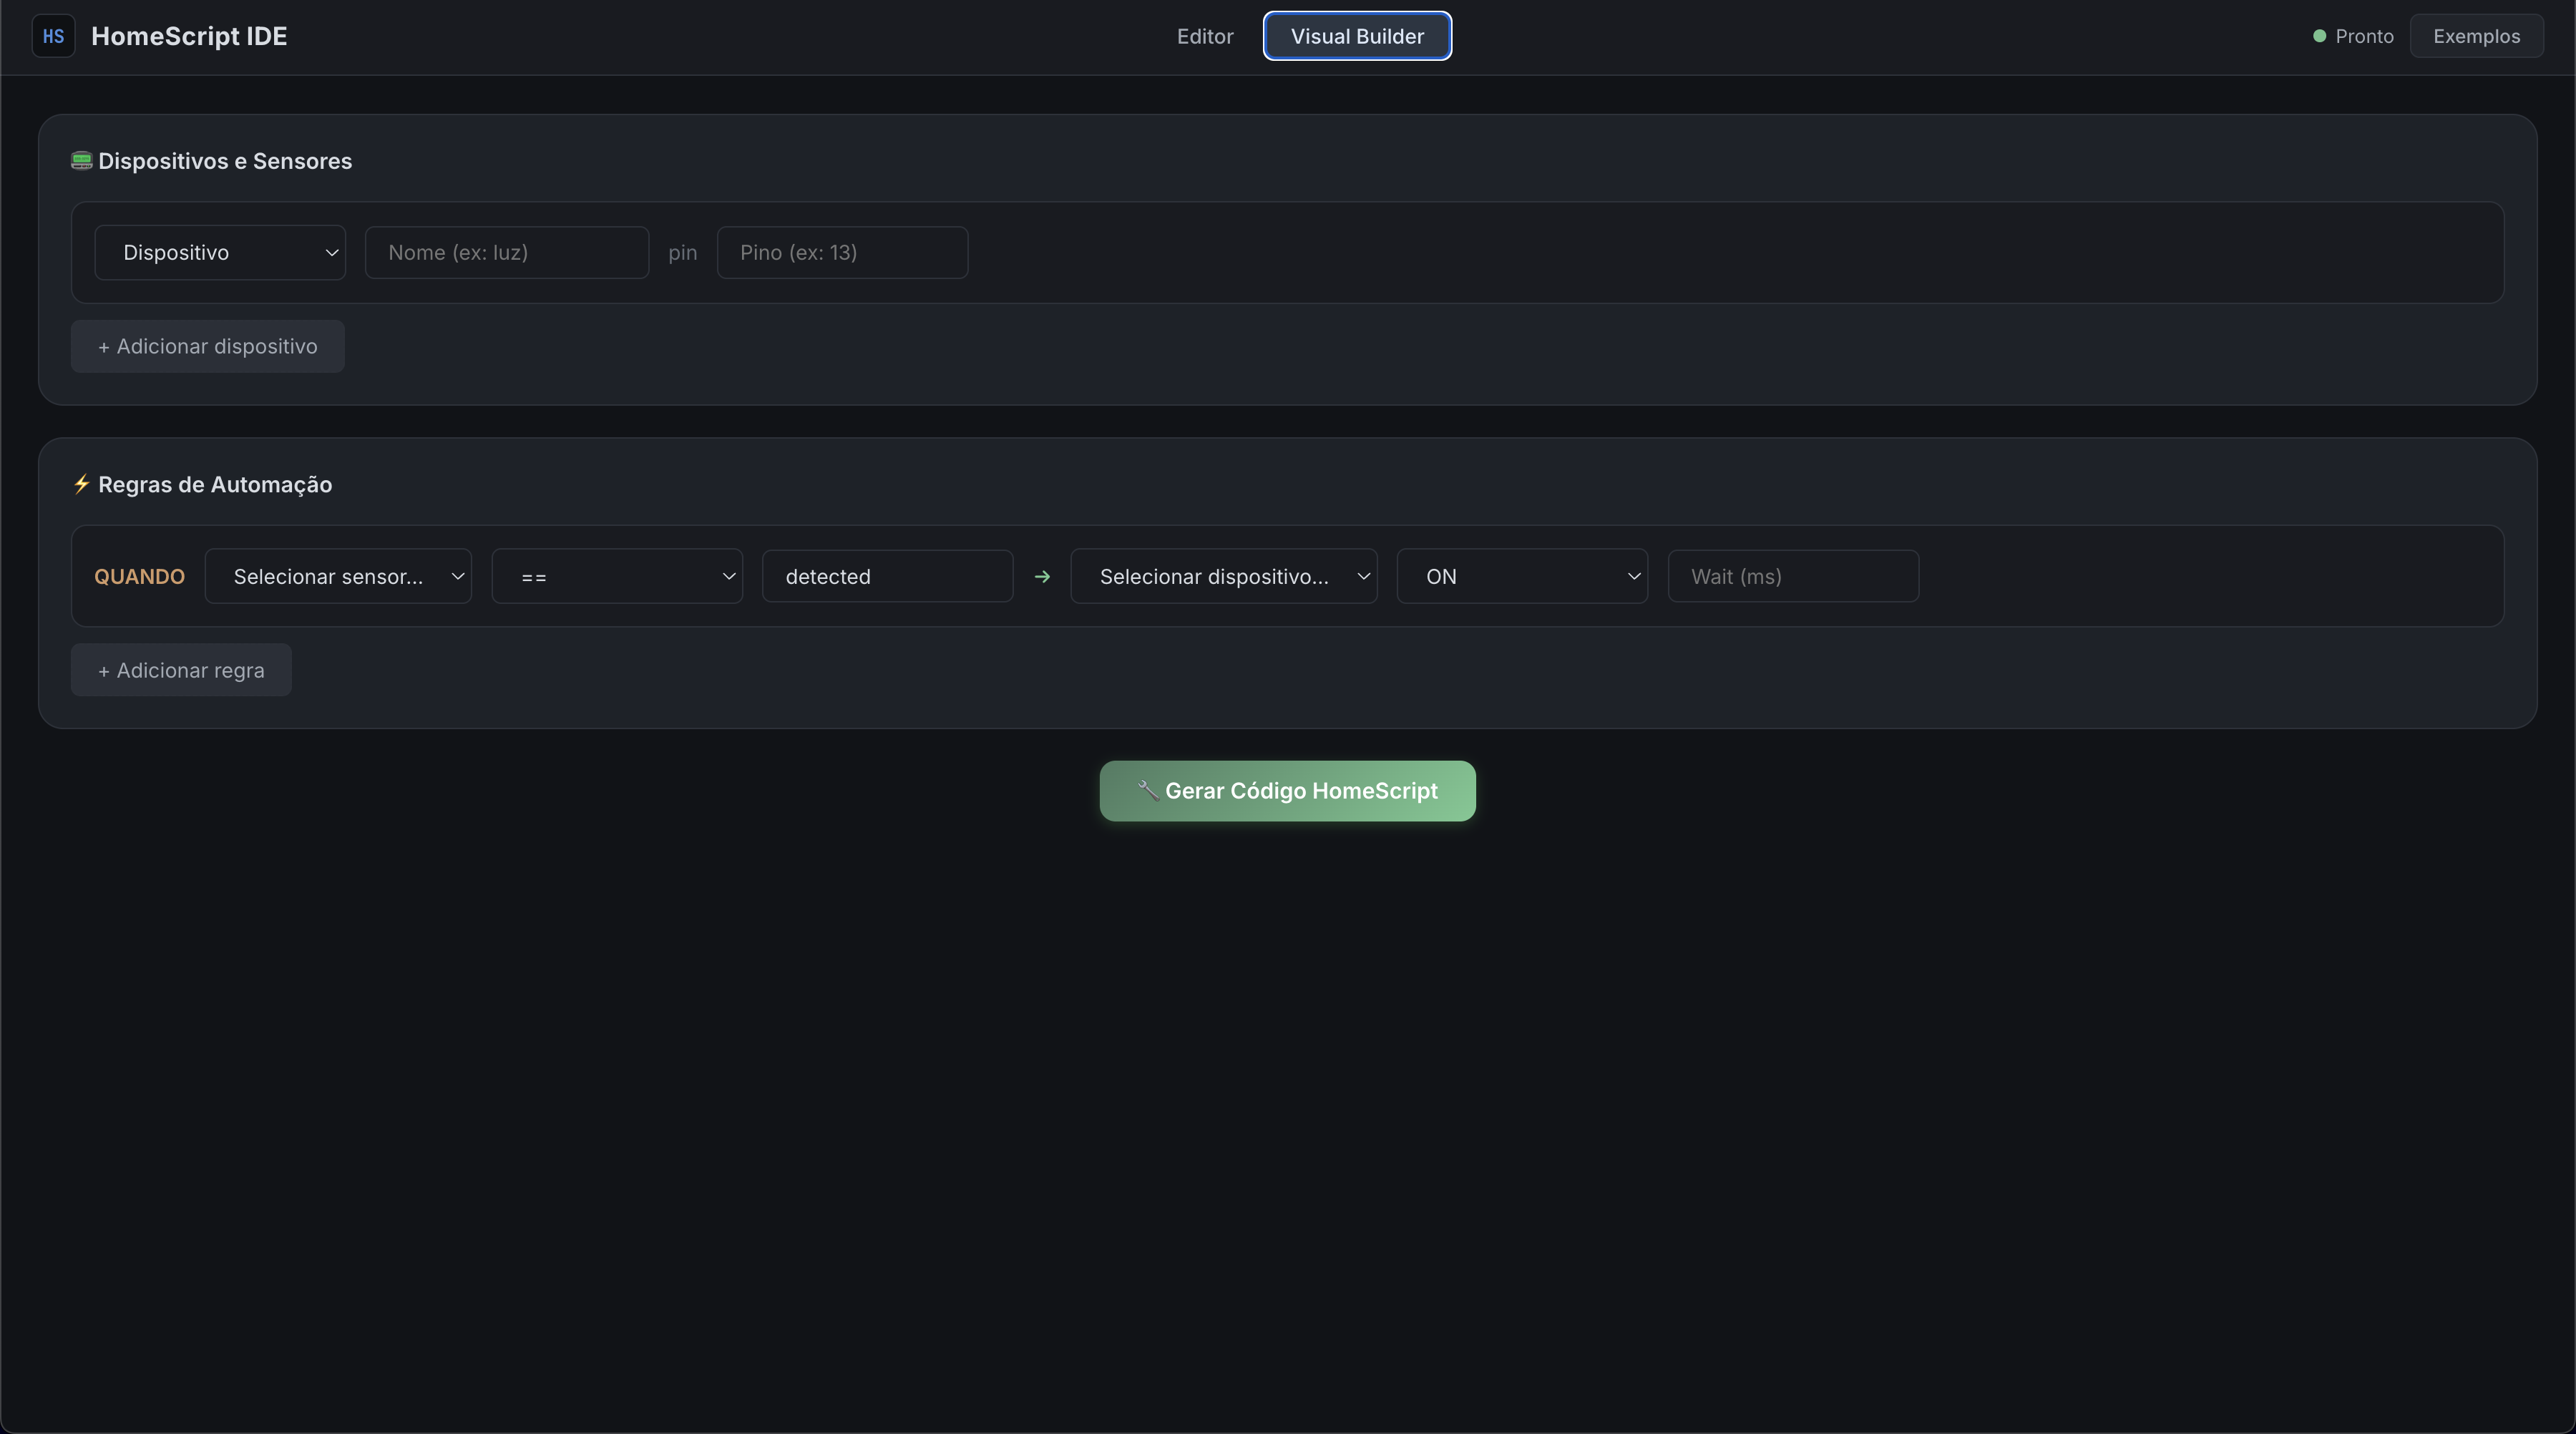
\includegraphics[width=0.95\linewidth]{../img/tela2.png}}
\caption{Visual Builder para montar automações sem escrever código manualmente.}
\label{fig:visual}
\end{figure}

O Monaco foi configurado com uma linguagem \texttt{homescript}: palavras-chave em inglês e português, comentários, números, operadores e delimitadores recebem destaque. O autocomplete oferece snippets para declarações, sensores DHT11, sensores HC-SR04, \texttt{if}, \texttt{when}, \texttt{for}, \texttt{while}, \texttt{wait}, \texttt{print} e atalhos em português. Também há sugestões de identificadores já declarados no código.

O painel de resultados possui quatro abas. A aba de código C mostra o resultado final. A aba de execução cria um rastro didático das fases do compilador, incluindo leitura de linhas, classificação de tokens e nós da AST. A aba de tokens exibe linha, coluna, tipo e valor. A aba AST mostra a estrutura retornada pelo backend. Em caso de erro, a interface apresenta a fase, linha, coluna e mensagem.

O Visual Builder oferece uma alternativa para usuários que não querem escrever código. Ele permite cadastrar dispositivos e sensores, criar regras com gatilho, operador, valor, ação, estado e espera opcional. Ao final, gera código HomeScript e retorna para o editor textual. Isso conecta a proposta acadêmica do compilador com uma experiência de produto mais acessível.

\section{Exemplos e Testes}
O repositório contém vários exemplos \texttt{.iot}: \texttt{teste.iot}, \texttt{sensor\_luz.iot}, \texttt{automacao\_completa.iot}, \texttt{dht11.iot}, \texttt{hcsr04.iot}, \texttt{teste2.iot} e \texttt{casa\_completa\_plus.iot}. Eles cobrem desde automações simples até cenários com múltiplos dispositivos, variáveis, sensores especializados, laços e comandos em português.

\begin{table}[htbp]
\caption{Cenários cobertos pelos exemplos}
\label{tab:exemplos}
\centering
\begin{tabular}{p{0.35\linewidth}p{0.55\linewidth}}
\toprule
\textbf{Arquivo} & \textbf{Cobertura} \\
\midrule
\texttt{teste.iot} & Movimento liga luz, espera e desliga. \\
\texttt{sensor\_luz.iot} & Sensor analógico com comparações numéricas. \\
\texttt{automacao\_completa.iot} & Múltiplos dispositivos, sensores e regras. \\
\texttt{dht11.iot} & Sensor de temperatura com biblioteca DHT. \\
\texttt{hcsr04.iot} & Sensor ultrassônico com \texttt{trig}/\texttt{echo}. \\
\texttt{casa\_completa\_plus.iot} & Sintaxe PT-BR, variáveis, \texttt{if/else}, \texttt{when/else}, \texttt{for}, \texttt{while}, DHT11 e HC-SR04. \\
\bottomrule
\end{tabular}
\end{table}

O \texttt{Makefile} do compilador possui alvos para compilar, limpar, executar testes padrão, testar apenas tokens, testar AST, testar JSON e gerar arquivo C. No frontend, os scripts incluem \texttt{npm run dev}, \texttt{npm run build}, \texttt{npm run lint} e \texttt{npm run preview}. O \texttt{docker-compose.yml} define serviços para backend e frontend, com portas \texttt{8000} e \texttt{5173}, facilitando demonstração integrada.

Durante o desenvolvimento, os principais problemas encontrados foram: sincronizar a gramática documentada com a gramática implementada, preservar linha e coluna corretas no lexer, diferenciar palavras reservadas de identificadores, representar expressões sem criar uma árvore aritmética completa, serializar AST em JSON para o frontend, tratar erros sem quebrar a resposta da API e mapear sensores diferentes para código Arduino adequado. A solução adotada foi manter o compilador modular e adicionar validações gradualmente, sempre com exemplos concretos para cada novo recurso. O walkthrough do projeto registra essa visão integrada de compilador, backend e frontend~\cite{docs-project}.

\section{Erros, Acertos e Depuração}
Um dos acertos do projeto foi manter a linguagem pequena no início. Isso permitiu entregar rapidamente um lexer funcional e uma demonstração com tokens. A partir desse núcleo, a equipe aumentou a linguagem com parser, variáveis, laços e sensores específicos. Outro acerto foi criar a saída JSON no próprio compilador, pois isso reduziu a complexidade da API e tornou o frontend apenas consumidor de um formato estruturado.

O principal erro de projeto evitado durante a evolução foi misturar responsabilidades. Se o backend tentasse implementar parte da análise da linguagem, o comportamento da CLI e da interface web poderia divergir. Por isso, a regra adotada foi manter a fonte da verdade no compilador em C. O backend apenas executa o binário e repassa a resposta. O frontend apenas apresenta os dados e ajuda o usuário a escrever código.

A depuração aconteceu em camadas. Quando havia erro léxico, a equipe verificava primeiro o token gerado, linha e coluna. Quando havia erro sintático, a AST era impressa para identificar onde o parser parava. Quando o código C era gerado incorretamente, o problema normalmente estava no mapeamento da AST para Arduino. No frontend, a aba de execução foi criada justamente para transformar esse processo de depuração em uma explicação visual do pipeline.

\section{Limitações}
Apesar de funcional, o HomeScript ainda possui limitações técnicas. Números são inteiros; não há strings literais; comentários são apenas de linha; expressões aritméticas são armazenadas como texto normalizado, não como uma subárvore de expressão completa; o buffer de código gerado possui tamanho máximo fixo; e a linguagem ainda não possui funções definidas pelo usuário. Além disso, o backend executa o compilador como subprocesso local, o que é simples para o projeto acadêmico, mas exigiria isolamento adicional em produção.

Outra limitação é que a diferença semântica entre \texttt{if} e \texttt{when} é pequena no código gerado atual, pois ambos viram \texttt{if} dentro do \texttt{loop()}. Para Arduino, isso funciona como avaliação contínua, mas uma evolução futura poderia tratar eventos e prioridades de forma mais explícita.

\section{Conclusão e Trabalhos Futuros}
O projeto atingiu o objetivo de criar uma linguagem própria para automação residencial e um pipeline completo de compilação. A solução implementa entrada \texttt{.iot}, lexer, parser, AST, análise semântica, geração de C/Arduino, CLI, saída JSON, backend FastAPI e frontend React com editor e builder visual. Dessa forma, o projeto demonstra conceitos centrais de compiladores e os aplica em um problema concreto.

O principal aprendizado foi que um compilador prático depende tanto da teoria das fases quanto de decisões de engenharia: mensagens de erro, formatos intermediários, testes, integração com ferramentas externas e experiência do usuário. O HomeScript mostra que uma DSL pequena, quando bem direcionada, pode esconder complexidade de baixo nível e tornar um domínio mais acessível.

Como trabalhos futuros, recomenda-se: adicionar literais de string e números decimais; criar uma AST própria para expressões aritméticas; expandir suporte a sensores e atuadores; gerar código para ESP32 com Wi-Fi/MQTT; criar simulador de execução; melhorar testes automatizados; adicionar persistência de projetos no frontend; permitir exportação direta do \texttt{.ino}; e reforçar segurança do backend para execução em ambiente compartilhado.

\section*{Agradecimentos}
A equipe agradece ao professor da disciplina de Compiladores pela orientação sobre a estrutura do artigo e pela exigência de uso do modelo IEEE, que guiou a organização deste relatório.

\balance
\begin{thebibliography}{00}
\bibitem{repo-readme} Projeto HomeScript, \textit{README.md}, repositório local do projeto, 2026.
\bibitem{docs-def} Projeto HomeScript, \textit{Definição da Linguagem HomeScript}, arquivo \texttt{docs/definicao\_linguagem.md}, 2026.
\bibitem{docs-lex} Projeto HomeScript, \textit{Manual Completo da Fase Léxica}, arquivo \texttt{docs/analise\_lexica\_manual.md}, 2026.
\bibitem{docs-tokens} Projeto HomeScript, \textit{Tabela de Tokens e Expressões Regulares}, arquivos \texttt{docs/tabela\_tokens.md} e \texttt{docs/regex.md}, 2026.
\bibitem{docs-project} Projeto HomeScript, \textit{Walkthrough do Projeto}, arquivo \texttt{docs/project.md}, 2026.
\bibitem{docs-front} Projeto HomeScript, \textit{Storyboard do Front-end}, arquivo \texttt{docs/storyboard\_frontend.md}, 2026.
\bibitem{arduino} Arduino, \textit{Arduino Language Reference}, disponível em \url{https://www.arduino.cc/reference/en/}.
\bibitem{fastapi} FastAPI, \textit{FastAPI Documentation}, disponível em \url{https://fastapi.tiangolo.com/}.
\bibitem{react} React, \textit{React Documentation}, disponível em \url{https://react.dev/}.
\bibitem{monaco} Microsoft, \textit{Monaco Editor Documentation}, disponível em \url{https://microsoft.github.io/monaco-editor/}.
\end{thebibliography}

\end{document}
